\documentclass[11pt, oneside]{article}   	% use "amsart" instead of "article" for AMSLaTeX format
\usepackage{geometry}                		% See geometry.pdf to learn the layout options. There are lots.
\geometry{letterpaper}                   		% ... or a4paper or a5paper or ... 
%\geometry{landscape}                		% Activate for for rotated page geometry
%\usepackage[parfill]{parskip}    		% Activate to begin paragraphs with an empty line rather than an indent
\usepackage{graphicx}				% Use pdf, png, jpg, or eps� with pdflatex; use eps in DVI mode
								% TeX will automatically convert eps --> pdf in pdflatex		
\usepackage{amssymb}
\usepackage{amsmath}

\title{Parametrizing Surfaces (Paul)}
%\author{The Author}
\date{}							% Activate to display a given date or no date

\graphicspath{{/Users/telliott_admin/Dropbox/Tex/png/}}
\begin{document}

\maketitle
%\section{}
% \subsection*{R code}
% \begin{lstlisting}  \end{lstlisting}
% \begin{center} 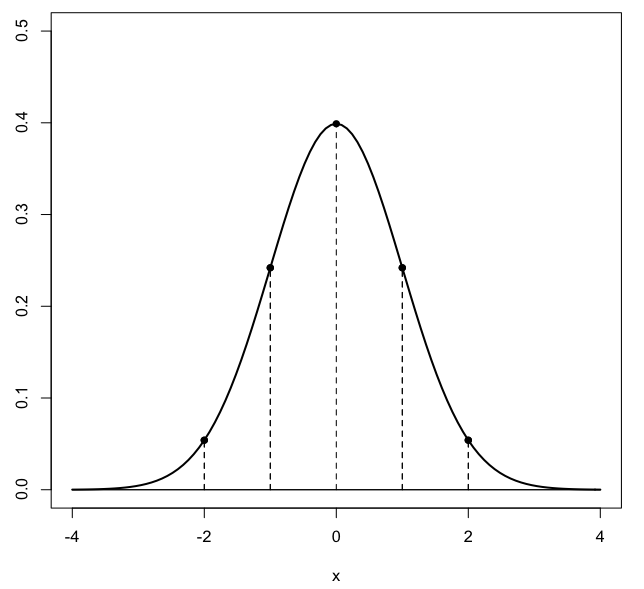
\includegraphics [scale=0.4] {gauss3.png} \end{center}
% \begin{bmatrix} a  &  b \\ c  &  d \end{bmatrix}
% \bigg |_

\large
\noindent
When we parametrized curves, we were able to work with curves where $x$,$y$ and $z$ were functions of a single parameter, which we usually call $t$.  For surfaces, we will usually have two variables $u$ and $v$.  For example, on the globe we locate our position by longitude and latitude.

As an example, consider
\[ \mathbf{r}(u,v) = u \hat{i} + u \ cos \ v \hat{j} + u \ sin \ v \hat{k} \]
We have three parametric equations, one for each variable

\[ x = u \]
\[ y = u \ cos \ v \]
\[ z = u \ sin \ v \]
So what this looks like is that we'll have a circle parallel to the yz-plane with radius $u$, where $u = x$.  We notice that if we square all the terms
\[ x^2 = u^2 \]
\[ y^2 + z^2 = u^2 \cos^2 \ v + u^2 \sin^2 \ v = u^2 = x^2 \]

Going from the equations back to the surface is fairly unusual.  Typically we do things the other way around.
\subsection*{Paraboloid}

Suppose we start with the elliptic paraboloid
\[ x = 5y^2 + 2z^2 - 10 \]
To visualize this, think about what happens when $x=0$.  Then we have an ellipse parallel to the $yz$-plane.  At $x=-10$, $y=z=0$;  and $x$ must be at least $-10$, because otherwise the squared terms would have to sum to less than zero, which is impossible with real numbers.

If we plot this
\begin{center} 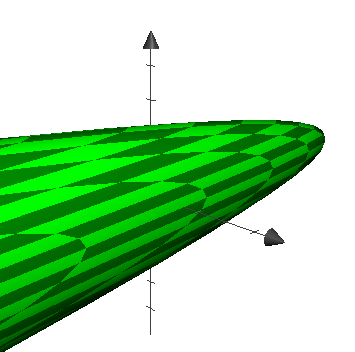
\includegraphics [scale=0.4] {param1.png} \end{center}

the paraboloid is symmetric around the x-axis (the cross-sections really are ellipses), and the vertex is at $x=-10$.  Here, we can pick $y$ and $z$ to be anything (there is a point on the surface for every $y,z$ pair).  $x$ is given by the equation above so
 
\[ \mathbf{r}(y,z) = (5y^2 + 2z^2 -10)\hat{i} + y \hat{j} + z \hat{k} \]

\subsection*{Sphere}
\[ x^2 + y^2 + z^2 = 16 \]
This is just a sphere of radius $4$.  The parametric representation uses the two angles $\phi$ and $\theta$.

\[ x = \rho \ sin \phi \ cos \theta \]
\[ y = \rho \ sin \phi \ sin \theta \]
\[ z = \rho \ cos \phi \]
where $\phi$ is the angle with respect to the positive z-axis.  So in the xy-plane
\[ \phi=\pi/2, \ \ cos \phi = 0, \ \ z = 0, \ \ x = \rho \ cos \theta, \ \ y = \rho \ sin \theta \]
and we just have a circle of radius $\rho$.  In fact, for any $z < \rho$, the angle $\phi$ is determined, which then makes the radius of the circle traced out by $x$ and $y$ smaller.

\[ \mathbf{r}(\theta,\phi) = \rho \ sin \phi \ cos \theta \ \hat{i} + \rho \ sin \phi \ sin \theta  \ \hat{j} + \rho \ cos \phi \ \hat{k} \]
\[ 0 \le \phi \le \pi, \ \ 0 \le \theta \le 2 \pi \]

\subsection*{Cylindrical coordinates}
\[ x^2 + y^2 = 25 \]
Now we have no restrictions on $z$.
\[ x = rcos \theta, \ \ y = rsin \theta, \ \ z = z \]
\[ \mathbf{r}(\theta,\phi) = rcos \theta \ \hat{i} + rsin \theta \ \hat{j} + z \hat{k} \]
\[ 0 \le \theta \le 2 \pi \]

\subsection*{Tangent plane}
A crucial idea is the method to find the equation of the tangent plane to a surface at a point.

\[ \mathbf{r}(u,v) = x(u,v) \ \hat{i} + y(u,v) \ \hat{j} + z(u,v) \  \hat{k} \]
The method is to find these two vectors
\[ \mathbf{r_u}(u,v) = \frac{\partial x}{\partial u}(u,v) \ \hat{i} + \frac{\partial y}{\partial u}(u,v) \ \hat{j} + \frac{\partial z}{\partial u}(u,v) \  \hat{k} \]
\[ \mathbf{r_v}(u,v) = \frac{\partial x}{\partial v}(u,v) \ \hat{i} + \frac{\partial y}{\partial v}(u,v) \ \hat{j} + \frac{\partial z}{\partial v}(u,v) \  \hat{k} \]
Now just form the cross product
\[ \mathbf{r_u} \times \mathbf{r_v} = \mathbf{n} \]
Provided $\mathbf{n} \ne 0$, this is the normal vector to the surface.

\subsection*{Example}
Suppose we have
\[ \mathbf{r}(u,v) = u \ \hat{i} + 2v^2 \ \hat{j} + (u^2 + v) \ \hat{k} \]
and we're looking at the point $(2,2,3)$.  We find the two tangent vectors using the equation above
\[ \mathbf{r_u} = \hat{i} + 2u \ \hat{k} = \ <1,0,2u> \]
\[ \mathbf{r_v} = 4v \ \hat{j} + \hat{k} = \ <0,4v,1> \]
The cross product is set up like this
\[
\begin{bmatrix}
\hat{i} & \hat{j} & \hat{k} \\
1 & 0 & 2u \\
0 & 4v & 1 
\end{bmatrix}
\]
so
\[ \mathbf{n} = -8uv \ \hat{i} - \hat{j} + 4v \ \hat{k} = \ <-8uv, -1, 4v> \]
So far so good, but now we need to solve for $u$ and $v$.  We plug the point we were given into the parametric equations
\[ x = u, \ \ y = 2v^2, \ \ z = u^2 + v \]
\[ 2 = u, \ \ 2 = 2v^2, \ \ 3 = u^2 + v \]
From the first two equations we get
\[ u = 2, v = \pm 1 \]
And the third equation restricts $v$ further
\[ v = -1 \]
So then the normal vector is
\[ \mathbf{n} = \ <16, -1, -4> \]
and the tangent plane is just
\[ 16(x-2) - (y-2) -4(z-3) = 0 \]
\[ 16x -y -4z = 18 \]
That was fairly painless!

\subsection*{Surface Area}
The surface area is given by
\[ A = \int \int_D \ \Vert \mathbf{r_u} \times \mathbf{r_v} \Vert \ dA \]
Consider a sphere of radius $a$
\[ x^2 + y^2 + z^2 = a^2 \]
If we parametrize this as before

\[ x = \rho \ sin \phi \ cos \theta = a \ sin \phi \ cos \theta \]
\[ y = \rho \ sin \phi \ sin \theta = a \ sin \phi \ sin \theta\]
\[ z = \rho \ cos \phi = a \ cos \phi \]

We can either remember that the normal vector at any point on this sphere is
\[ \mathbf{n} = \ <x, y, z> \]
or we can write
\[ \mathbf{r}(\theta,\phi) = a \ sin \phi \ cos \theta \ \hat{i} + a \ sin \phi \ sin \theta \ \hat{j} + a \ cos \phi \ \hat{k} \]
\[ \mathbf{r_{\theta}} = - a\ sin \phi \ sin \theta \ \hat{i} + a \ sin \phi \ cos \theta \  \hat{j} + 0 \ \hat{k} \]
\[ \mathbf{r_{\phi}} = a\ cos \phi \ cos \theta \ \hat{i} + a \ cos \phi \ sin \theta \  \hat{j} - a \ sin \phi \ \hat{k} \]
And
\[ \mathbf{N} = \mathbf{r_{\theta}} \times \mathbf{r_{\phi}} = a^2
\begin{bmatrix}
\hat{i} & \hat{j} & \hat{k} \\
-sin \phi \ sin \theta & sin \phi \ cos \theta & 0 \\
\ \ cos \phi \ cos \theta & cos \phi \ sin \theta & -sin \ \phi 
\end{bmatrix}
\]
the components are (all multiplied by $a^2$) and then we have
\[ -sin^2\phi \ cos \ \theta \  \hat{i} \]
\[ -sin^2\phi \ sin \ \theta \  \hat{j} \]
\[ -sin\phi \ cos\phi \ sin^2\theta - sin\phi \ cos\phi \ cos^2\theta \  \hat{k} = -sin \phi \ cos \phi \  \hat{k} \]

\[ \mathbf{N} = a^2 \ sin \phi \ <-sin \phi \ cos \theta, -sin \phi \ sin \theta, -cos \phi > \]
\[ \Vert \mathbf{N} \Vert = a^2 \ sin \phi \ \sqrt{sin^2\phi \ cos^2\theta + sin^2\phi \ sin^2\theta + cos^2\phi } \]
\[ \Vert \mathbf{N} \Vert = a^2 \ sin \phi \ \sqrt{sin^2\phi  + cos^2\phi } = a^2 \ sin \phi\]
\[ \mathbf{n} = \mathbf{N} / \Vert \mathbf{N} \Vert = \ <-sin \phi \ cos \theta, -sin \phi \ sin \theta, -cos \phi > \]
This is the unit normal at the point
\[ (a \ sin \phi \ cos \theta, a \ sin \phi \ sin \theta, a \ cos \phi ) = (x,y,z) \]
The sign of the normal vector is negative.  By convention $\mathbf{n}$ points into the sphere.

How do we integrate this to get the surface area?  Aren't we mixing up $x,y,z$ with $\theta,\phi$?  The answer is that in this formula
\[ A = \int \int_D \ \Vert \mathbf{r_{\theta}} \times \mathbf{r_{\phi}} \Vert \ dA = \int \int_D \ \Vert \mathbf{N} \Vert \ dA = \int \int_D \ a^2 \ sin \phi \ dA \]
 $dA = \ d\theta \ d\phi$.  It is not really the area element, because we need to correct by using the Jacobian, which is what we really just computed above..
 The area element is actually $a^2 \ sin \phi \ d\theta \ d\phi$.
 \[ A = \int \int_D \ a^2 \ sin \phi \ d\theta \ d\phi \]
\[ 0 \le \phi \le \pi, \ \ 0 \le \theta \le 2 \pi \]
\[ A = \int_0^{\pi} \int_0^{2\pi} \ a^2 \ sin \phi \ d\theta \ d\phi \]
The inner integral is
\[ \int_0^{2\pi} \ a^2 \ sin \phi \ d\theta = 2 \pi a^2 \ sin \phi \]
and the outer integral is then
\[ \int_0^{\pi} 2 \pi a^2 \ sin \phi \  d \phi = 2\pi a^2 (-1)(cos \phi) \bigg |_0^{\pi} =  2\pi a^2 (-1)(-2) = 4\pi a^2 \]
which is correct.

\subsection*{Formulas (Marsden)}
We don't actually have to set up the cross product as the determinant, because we are going to get the norm (magnitude) of it right away.

\[ \Vert \mathbf{r_{\theta}} \times \mathbf{r_{\phi}} \Vert = \sqrt{(\frac{\partial (x,y)}{\partial (u,v)})^2 + (\frac{\partial (y,z)}{\partial (u,v)})^2 + (\frac{\partial (x,z)}{\partial (u,v)})^2}\]

where
\Large
\[ \frac{\partial (y,z)}{\partial (u,v)}) = 
\begin{vmatrix}
\frac{\partial x}{\partial u} & \frac{\partial x}{\partial v} \\
\frac{\partial y}{\partial u} & \frac{\partial y}{\partial v}
\end{vmatrix}
\]
\large
and so on.  This is our old friend, the Jacobian.  Thus, the area formula becomes
\[ A = \int \int_R \sqrt{(\frac{\partial (x,y)}{\partial (u,v)})^2 + (\frac{\partial (y,z)}{\partial (u,v)})^2 + (\frac{\partial (x,z)}{\partial (u,v)})^2} \ du \ dv \]

\subsection*{One more}
I have one more example from Paul.  He says:  find the surface area of the portion of the sphere of radius $4$ that lies inside the cylinder $x^2 + y^2 = 12$ and above the xy-plane.

This shape is called a "spherical cap."  The problem should be pretty easy because we just worked out the area element for the sphere above.  We have 
\[ A = \int \int_D \ a^2 \ sin \phi \ d\theta \ d\phi \]
The trick is to find out where the cylinder and the sphere intersect.  We have 
\[ x^2 + y^2 + z^2 = 16 \]
\[ x^2 + y^2 = 12 \]
These are both true when $z^2 = 4, z = \pm \ 2$.
What we need to do is to find the angle $\phi$ that this corresponds to.  Since we know that
\[ z = a \ cos \phi, \ \ a = 4, \ \ z=2 \]
\[ cos \phi = \frac{1}{2}, \ \ \phi = \frac{\pi}{3} \]
So we have that the range of $\phi$ is
\[ 0 \le \phi \le \frac{\pi}{3} \]
Remember that $\phi = 0$ at the top of the sphere, and that's the part we want, above the circle formed by the intersection of the cylinder and the sphere.

\[ A =  \int_0^{\pi/3} \int_0^{2\pi} \ a^2 \ sin \phi \ d\theta \ d\phi \]
The inner integral is 
\[ \int_0^{2\pi} \ a^2 \ sin \phi \ d\theta = 2\pi a^2 \ sin \phi \]
and the outer is
\[  \int_0^{\pi/3} 2\pi a^2 \ sin \phi   \ d\phi \]
\[  2\pi a^2 \ (-cos \phi) \ \bigg |_0^{\pi/3} = 2\pi a^2 (-\frac{1}{2} + 1) = \pi a^2 = 16 \pi \]



\end{document}  